% =========================================================================
%  pycorrect -- User manual
%  Python translation of CORRECT 2.24 (Howe, McGreevy, Zetterstrom)
%  Compile with:  pdflatex pycorrect_manual.tex   (twice, for the TOC)
%  Figures are produced by  python make_figures.py
% =========================================================================
\documentclass[11pt,a4paper]{report}

\usepackage[T1]{fontenc}
\usepackage[utf8]{inputenc}
\usepackage{mathpazo}
\usepackage{courier}
\usepackage{microtype}
\usepackage[a4paper,margin=2.5cm,headheight=14pt]{geometry}
\usepackage{amsmath,amssymb}
\usepackage{graphicx}
\usepackage{booktabs,tabularx,longtable,array}
\usepackage{xcolor}
\usepackage{listings}
\usepackage[most]{tcolorbox}
\usepackage{enumitem}
\usepackage{fancyhdr}
\usepackage{titlesec}
\usepackage{caption}
\usepackage{float}
\usepackage{tikz}
\usetikzlibrary{arrows.meta,positioning,shapes.geometric}
\usepackage[colorlinks=true,linkcolor=accent,urlcolor=accent,citecolor=accent]{hyperref}

% ---------------------------------------------------------------- colours
\definecolor{accent}{HTML}{2A78D6}
\definecolor{accent2}{HTML}{EB6834}
\definecolor{accent3}{HTML}{1BAF7A}
\definecolor{ink2}{HTML}{52514E}
\definecolor{codebg}{HTML}{F6F6F4}
\definecolor{noteback}{HTML}{EEF4FC}
\definecolor{warnback}{HTML}{FDF0EA}

% ---------------------------------------------------------------- headings
\titleformat{\chapter}[display]{\normalfont\bfseries\color{accent}}
  {\large\scshape \chaptertitlename\ \thechapter}{4pt}{\Huge}
\titlespacing*{\chapter}{0pt}{-20pt}{24pt}
\titleformat{\section}{\normalfont\Large\bfseries\color{accent}}{\thesection}{0.8em}{}
\titleformat{\subsection}{\normalfont\large\bfseries}{\thesubsection}{0.8em}{}

\pagestyle{fancy}
\fancyhf{}
\fancyhead[L]{\small\color{ink2}\textsc{pycorrect} user manual}
\fancyhead[R]{\small\color{ink2}\nouppercase{\leftmark}}
\fancyfoot[C]{\small\thepage}
\renewcommand{\headrulewidth}{0.4pt}

% ---------------------------------------------------------------- code
\lstdefinestyle{base}{
  basicstyle=\ttfamily\small, backgroundcolor=\color{codebg},
  frame=single, rulecolor=\color{codebg}, framesep=4pt, xleftmargin=4pt,
  xrightmargin=4pt, breaklines=true, columns=fullflexible, keepspaces=true,
  showstringspaces=false, aboveskip=8pt, belowskip=8pt,
  commentstyle=\color{ink2}\itshape, keywordstyle=\color{accent}\bfseries,
  stringstyle=\color{accent2}, upquote=true}
\lstdefinelanguage{com}{
  morekeywords={background,beam,cadmium,calibration,collimator,component,
    container,execute,faithful,furnace,geometry,instrument,list,low_angle,
    monitor,output,placzek,quit,range,sample,spectrum,title,vanadium,
    wavelength,write,xin,xout},
  sensitive=false, morecomment=[l]{!}, morestring=[b]"}
\lstnewenvironment{com}[1][]{\lstset{style=base,language=com,#1}}{}
\lstnewenvironment{py}[1][]{\lstset{style=base,language=Python,#1}}{}
\lstnewenvironment{shell}[1][]{\lstset{style=base,#1}}{}
\lstnewenvironment{out}[1][]{\lstset{style=base,basicstyle=\ttfamily\scriptsize,#1}}{}
\newcommand{\cmd}[1]{\texttt{\color{accent}#1}}
\newcommand{\code}[1]{\texttt{#1}}
\newcommand{\file}[1]{\texttt{#1}}

% ---------------------------------------------------------------- boxes
\newtcolorbox{note}[1][Note]{colback=noteback,colframe=accent,boxrule=0pt,
  leftrule=3pt,arc=0pt,fonttitle=\bfseries,coltitle=accent,colbacktitle=noteback,
  title=#1,attach title to upper={\ \ },before skip=8pt,after skip=8pt}
\newtcolorbox{warn}[1][Caution]{colback=warnback,colframe=accent2,boxrule=0pt,
  leftrule=3pt,arc=0pt,fonttitle=\bfseries,coltitle=accent2,colbacktitle=warnback,
  title=#1,attach title to upper={\ \ },before skip=8pt,after skip=8pt}
\newtcolorbox{cmdbox}[1]{colback=white,colframe=accent,boxrule=0.6pt,arc=2pt,
  fonttitle=\ttfamily\bfseries,coltitle=white,title={#1},before skip=10pt,after skip=6pt}

\setlist{itemsep=2pt,topsep=4pt}
\captionsetup{font=small,labelfont={bf,color=accent}}
\setlength{\parindent}{0pt}
\setlength{\parskip}{5pt}

\newcommand{\pyc}{\textsc{pycorrect}}
\newcommand{\cor}{\textsc{correct}}
\newcommand{\dsig}{\frac{d\sigma}{d\Omega}}

% =========================================================================
\begin{document}

% ---------------------------------------------------------------- title
\begin{titlepage}
\thispagestyle{empty}
\vspace*{2.5cm}
{\color{accent}\rule{\linewidth}{2pt}}\par\vspace{0.6cm}
{\fontsize{44}{48}\selectfont\bfseries\pyc}\par\vspace{0.3cm}
{\LARGE Corrections for neutron diffraction data}\par\vspace{0.2cm}
{\Large\color{ink2} Attenuation (Paalman \& Pings), multiple scattering
(Blech \& Averbach), Placzek and vanadium normalisation}\par
\vspace{0.6cm}{\color{accent}\rule{\linewidth}{2pt}}\par
\vspace{1.5cm}
{\Large User Manual}\par\vspace{0.3cm}
{\large Version 2.24.0 \quad(Python translation of \cor\ 2.24)}\par
\vfill
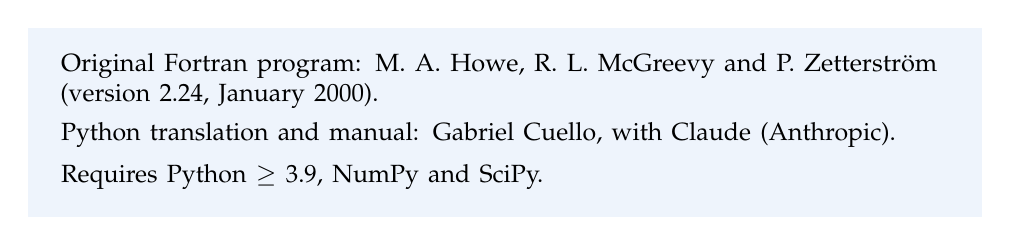
\begin{tikzpicture}
  \fill[noteback] (0,0) rectangle (\linewidth,2.4);
  \node[anchor=north west,text width=0.95\linewidth,align=left] at (0.3,2.2) {
  \small Original Fortran program: M.~A.~Howe, R.~L.~McGreevy and
  P.~Zetterstr\"om (version 2.24, January 2000).\\[3pt]
  Python translation and manual: Gabriel Cuello, with Claude (Anthropic).\\[3pt]
  Requires Python $\geq$ 3.9, NumPy and SciPy.};
\end{tikzpicture}
\vspace{1cm}
{\small\color{ink2}\today}
\end{titlepage}

\pagenumbering{roman}
\tableofcontents
\clearpage
\pagenumbering{arabic}

% =========================================================================
\chapter{Introduction}
% =========================================================================

\pyc\ is a Python version of \cor, the program written by
M.~A.~Howe, R.~L.~McGreevy and P.~Zetterstr\"om to turn the raw counts of a neutron
diffraction experiment into an absolute differential cross-section
$\dsig(Q)$. It handles constant-wavelength (two-axis) instruments such as
D4 and D20 at the ILL, and time-of-flight instruments such as LAD and SANDALS.

For each detector group (``spectrum'') the program:
\begin{enumerate}
  \item subtracts the empty-instrument background from every measurement;
  \item removes the scattering of the container and of the furnace or cryostat
        shield, using the \textbf{Paalman \& Pings} attenuation factors;
  \item corrects the vanadium (or the container, if there is no vanadium) for
        attenuation, \textbf{multiple scattering} (Blech \& Averbach) and
        the \textbf{Placzek} inelasticity effect, smooths it, and uses it to put
        the sample on an absolute scale;
  \item removes the multiple scattering of the sample and adds its Placzek
        correction;
  \item writes $\dsig$ as a function of $Q$ (or $2\theta$).
\end{enumerate}

\pyc\ keeps the command language of \cor: an old command file (\file{.com})
runs unchanged. It also exposes every intermediate quantity to Python, so you can
compare the analytical corrections, step by step, with a Monte Carlo simulation
of the neutron trajectories, such as the AMS (Attenuation and Multiple
Scattering) code.

\section{What is in the package}

\begin{center}
\begin{tabularx}{\linewidth}{@{}lX@{}}
\toprule
Path & Content \\
\midrule
\file{pycorrect/} & the Python package (one module per Fortran file, see Appendix~\ref{app:corr}) \\
\file{pycorrect/doublescattering.dat} & Blech \& Averbach table of $\delta_2(\mu R, R/H)$ \\
\file{pycorrect/xsect.dat} & neutron cross-sections and atomic weights of the elements \\
\file{examples/make\_d4\_example.py} & builds a synthetic D4 data set with a known answer \\
\file{examples/pp\_factors\_table.py} & tabulates the attenuation factors and $\delta$ for any geometry \\
\file{tests/test\_pycorrect.py} & self-tests (independent integration, round trip) \\
\file{manual/} & this manual and the script that makes its figures \\
\file{README.md} & short summary, list of the bugs of \cor\ 2.24 \\
\bottomrule
\end{tabularx}
\end{center}

\section{Conventions}

\begin{itemize}
  \item Lengths in \textbf{cm}, number densities in \textbf{atoms\,\AA$^{-3}$},
        cross-sections in \textbf{barn}, wavelengths in \textbf{\AA}, angles in
        \textbf{degrees} (the scattering angle is always the full $2\theta$).
  \item Absorption cross-sections are given at $\lambda_0 = 1.798$~\AA\
        (2200~m/s); the program scales them as $\sigma_a(\lambda) =
        \sigma_a\,\lambda/1.798$.
  \item Indices: $s$ sample, $c$ container (can), $h$ heater (furnace or
        cryostat shield), $v$ vanadium.
  \item In the commands, \cmd{monospace blue} words are verbs, words starting
        with \code{/} are qualifiers.
\end{itemize}

% =========================================================================
\chapter{Installation and first run}
% =========================================================================

\section{Requirements}

Python 3.9 or newer, with NumPy and SciPy. Matplotlib is only needed to rebuild
the figures of this manual.

\begin{shell}
pip install numpy scipy
\end{shell}

\section{Installing}

Unzip \file{pycorrect.zip} and install it in ``editable'' mode, so that changes
to the source take effect immediately:

\begin{shell}
unzip pycorrect.zip
cd pycorrect
pip install -e .
\end{shell}

This also creates the command \code{pycorrect}. If you prefer not to install,
add the top folder to \code{PYTHONPATH}:

\begin{shell}
export PYTHONPATH=/path/to/pycorrect:$PYTHONPATH      # Linux / macOS
set PYTHONPATH=C:\path\to\pycorrect;%PYTHONPATH%      # Windows
\end{shell}

Check the installation with the self-tests:

\begin{shell}
python tests/test_pycorrect.py
ok  test_paalman_pings_vs_brute_force
ok  test_mscat_limits
ok  test_parser
ok  test_roundtrip_2axis
\end{shell}

\section{Running}

There are three ways to use the program.

\paragraph{1. With a command file} (the usual way):
\begin{shell}
cd my_experiment            # file names in the .com file are relative to here
pycorrect run.com           # or: python -m toscana.corrections.pycorrect run.com
pycorrect @run              # same; ".com" is added when there is no extension
\end{shell}

\paragraph{2. Interactively.} Without arguments the program shows the prompt
\code{CORRECT>}; type commands one by one, \code{@file} runs a command file,
\cmd{quit} leaves.

\paragraph{3. From Python} (scripts, notebooks, comparisons with Monte Carlo):
\begin{py}
from toscana.corrections.pycorrect import Correct
c = Correct()
c.run_file("run.com")
r = c.results[0]          # all arrays of spectrum 1
\end{py}
Chapter~\ref{chap:python} describes this interface.

\section{A first example in five minutes}

The package can build a complete synthetic D4 experiment (nickel in a vanadium
can) whose true cross-section is known, so you can check the whole chain.

\begin{shell}
python examples/make_d4_example.py     # writes examples/d4_data/
cd examples/d4_data
pycorrect d4_example.com
\end{shell}

The command file it creates is:

\lstinputlisting[style=base,language=com]{listings/d4_example.com}

The corrected data are in \file{corrected.dat}; the true answer is in
\file{true\_dcs.txt}. Figure~\ref{fig:d4result} compares them; the agreement is
limited only by the Poisson noise put in the synthetic counts. Chapter~\ref{chap:examples}
explains every line.

\begin{figure}[H]
  \centering
  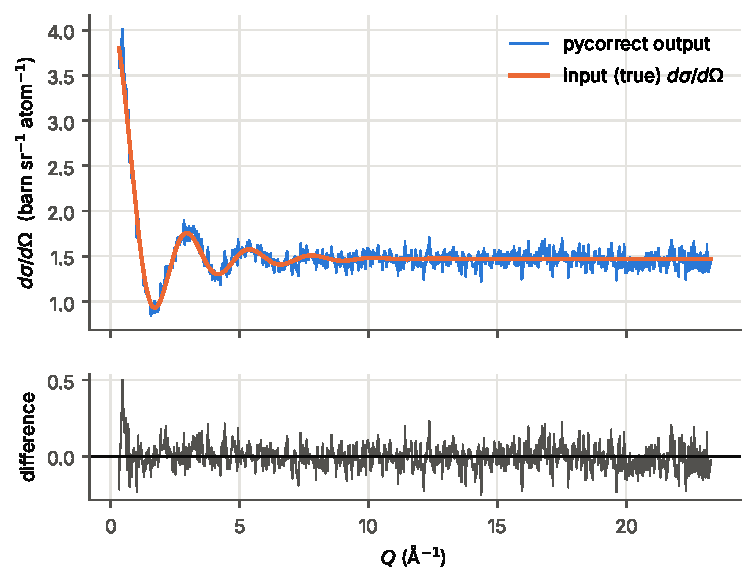
\includegraphics[width=0.85\linewidth]{figures/d4_result.pdf}
  \caption{Synthetic D4 example: output of \pyc\ (blue) and the cross-section
  used to build the raw data (orange). Lower panel: difference.}
  \label{fig:d4result}
\end{figure}

% =========================================================================
\chapter{Physical background}
\label{chap:physics}
% =========================================================================

This chapter summarises the formulae used by the program, with the name of the
function that implements each one.

\section{Measured intensities}

Consider a cylindrical sample (radius $R_1$) in a container (outer radius
$R_2$), inside a furnace or cryostat shield (radii $R_3 < R_4$). After the
empty-instrument background is subtracted, the intensities measured with the
furnace alone ($I_h$), with the empty container ($I_{ch}$) and with the full
container ($I_{sch}$) are
\begin{align}
  I^{\text{meas}}_{h}   &= A_{h,h}\, I_h, \\
  I^{\text{meas}}_{ch}  &= A_{c,ch}\, I_c + A_{h,ch}\, I_h, \\
  I^{\text{meas}}_{sch} &= A_{s,sch}\, I_s + A_{c,sch}\, I_c + A_{h,sch}\, I_h ,
\end{align}
where $I_s, I_c, I_h$ are the intensities that each body would scatter
without any attenuation. The program inverts these relations
(\code{correct\_2axis}):
\begin{align}
  I_h &= I^{\text{meas}}_{h} / A_{h,h}, \\
  I_c &= \bigl(I^{\text{meas}}_{ch} - A_{h,ch} I_h\bigr) / A_{c,ch}, \\
  I_s &= \bigl(I^{\text{meas}}_{sch} - A_{c,sch} I_c - A_{h,sch} I_h\bigr) / A_{s,sch}.
\end{align}

\section{Paalman \& Pings attenuation factors}

The notation is that of Paalman and Pings~\cite{pp}: the first index is the body
where the neutron is scattered; the indices after the comma are the bodies that
attenuate it on its way in and out. For a scattering point $\mathbf r$ in body
$i$ (cross-section area $S_i$),
\begin{equation}
  A_{i,jk\ldots}(2\theta) = \frac{1}{S_i}\int_{S_i}
  \exp\Bigl[-\sum_{m} \mu_m \bigl(l^{\text{in}}_m(\mathbf r) + l^{\text{out}}_m(\mathbf r, 2\theta)\bigr)\Bigr]
  \,dS ,
\end{equation}
where $l^{\text{in}}_m$ and $l^{\text{out}}_m$ are the path lengths in body $m$
before and after scattering, and
\begin{equation}
  \mu_m = n_m\,\bigl[\sigma_{s,m} + \sigma_{a,m}\,\lambda/1.798\bigr]
\end{equation}
is the total linear attenuation coefficient (cm$^{-1}$; $n$ in \AA$^{-3}$ and
$\sigma$ in barn give $\mu$ in cm$^{-1}$ directly since 1~barn\,\AA$^{-3}$ = 1~cm$^{-1}$).

\pyc\ evaluates the integrals as in \cor\ (function \code{atcors}):
\begin{itemize}
  \item polar coordinates $(r,\omega)$, 9-point Gauss--Legendre quadrature in both;
  \item a beam narrower than the sample or the can is allowed (points outside the beam get zero weight);
  \item the furnace factors are computed at $2\theta = 0^\circ, 90^\circ, 180^\circ$ and interpolated with a parabola;
  \item optionally, the transmission of an oscillating radial collimator is included (command \cmd{collimator});
  \item during a correction (function \code{absor}) the factors are computed at 10 angles and a 4th-degree polynomial in $2\theta$ is fitted to each one.
\end{itemize}
For flat plates, \code{plate} uses the analytical expressions for slabs.
Figure~\ref{fig:pp} shows the factors for the example of Chapter~2.

\begin{figure}[H]
  \centering
  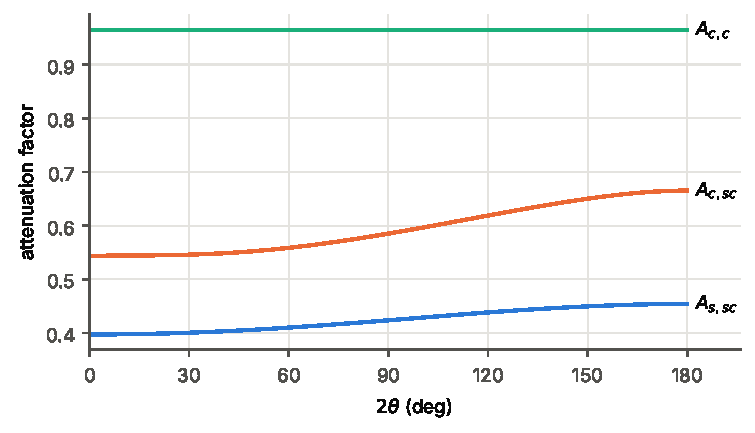
\includegraphics[width=0.85\linewidth]{figures/pp_factors.pdf}
  \caption{Paalman \& Pings factors for a Ni sample ($R_1=0.30$~cm) in a V can
  ($R_2=0.32$~cm), $\lambda=0.4985$~\AA, beam width 1.5~cm.}
  \label{fig:pp}
\end{figure}

\section{Multiple scattering (Blech \& Averbach)}

The ratio of multiply to singly scattered intensity in a cylinder of radius $R$
illuminated over a height $H$ is taken from Blech and Averbach~\cite{ba}. The
table \file{doublescattering.dat} gives the double-to-single ratio
$\delta_2(\mu R, R/H)$ (Figure~\ref{fig:ba}). Function \code{mscat}
\begin{enumerate}
  \item interpolates $\delta_2$ in the table (outside it, \code{mulscs}
        computes it by direct numerical integration);
  \item multiplies by the probability that the second event is a scattering,
        $d = \delta_2\,\mu_s/\mu_t$;
  \item adds the higher orders with the empirical series
  \begin{equation}
    \delta = d + 0.6940\,d^2 + 0.3701\,d^3 + 0.1605\,d^4 + 0.0587\,d^5 .
  \end{equation}
\end{enumerate}
$\delta$ does not depend on angle (isotropic approximation). For the sample in
its container, \pyc\ uses an effective cylinder of radius $R_2$ with
volume-averaged coefficients
$\bar\mu = (1-f)\mu_c + f\mu_s$, $f=(R_1/R_2)^2$.

\begin{figure}[H]
  \centering
  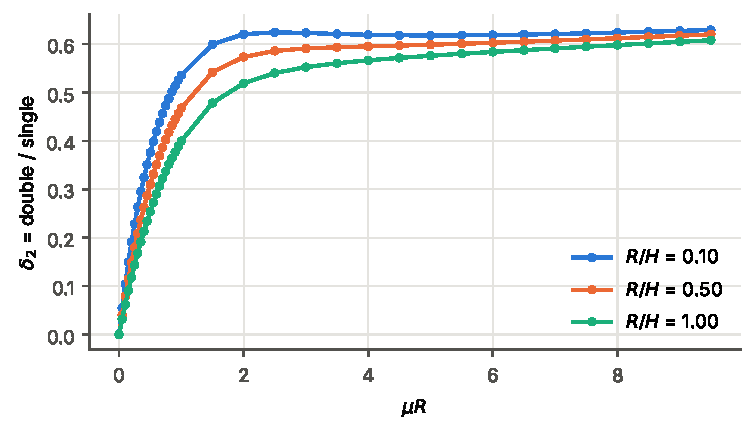
\includegraphics[width=0.85\linewidth]{figures/blech_averbach.pdf}
  \caption{Blech \& Averbach double-to-single scattering ratio from
  \file{doublescattering.dat}.}
  \label{fig:ba}
\end{figure}

\section{Placzek correction}

Because the nuclei recoil, the self scattering differs from $\sigma_s/4\pi$
by a $Q$-dependent amount $P$. For reactor instruments \code{placzek} uses the
expansion of Yarnell et al.~\cite{yarnell} (\cmd{placzek series}) or the
effective temperature of a vibrating diatomic molecule (\cmd{placzek diatomic}),
with detector-efficiency constants for D4, D20 and SLAD. For time-of-flight
instruments the expansions include the incident spectrum and detector
efficiency (\code{plaatom}, \code{plamol}).

\section{Normalisation to vanadium}

The vanadium rod (radius $R_v$) is corrected for attenuation, multiple
scattering and Placzek,
\begin{equation}
  I_v = \frac{I^{\text{meas}}_v}{A_{v,v}\,\bigl(1 - P_v + \delta_v\bigr)},
\end{equation}
smoothed (Bragg peaks of V removed), and used to normalise the sample:
\begin{equation}
  \dsig = \frac{I_s}{I_v}\,
          \frac{n_v R_v^2\,\sigma_{s,v}/4\pi}{n_s R_1^2}
          \;-\;\delta_s\,\frac{\sigma_{s}}{4\pi} \;+\; P_s ,
  \label{eq:norm}
\end{equation}
in barn\,sr$^{-1}$ per atom. Without vanadium the container, corrected the same
way, plays its role (factor $n_c(R_2^2-R_1^2)\sigma_{s,c}/4\pi$).

\section{Overview of the chain}

\begin{figure}[H]
\centering
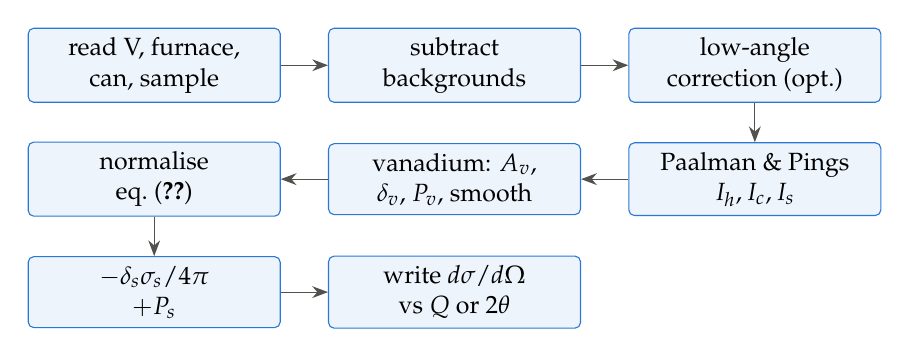
\begin{tikzpicture}[node distance=5mm and 6mm,
  box/.style={draw=accent,fill=noteback,rounded corners=2pt,minimum width=3.2cm,
              minimum height=7mm,align=center,font=\small},
  arr/.style={-{Stealth[length=2mm]},draw=ink2}]
\node[box] (read) {read V, furnace,\\ can, sample};
\node[box,right=of read] (bkg) {subtract\\ backgrounds};
\node[box,right=of bkg] (low) {low-angle\\ correction (opt.)};
\node[box,below=of low] (pp) {Paalman \& Pings\\ $I_h, I_c, I_s$};
\node[box,left=of pp] (van) {vanadium: $A_v$,\\ $\delta_v$, $P_v$, smooth};
\node[box,left=of van] (norm) {normalise\\ eq.~(\ref{eq:norm})};
\node[box,below=of norm] (ms) {$-\delta_s\sigma_s/4\pi$\\ $+P_s$};
\node[box,right=of ms] (out) {write $d\sigma/d\Omega$\\ vs $Q$ or $2\theta$};
\draw[arr] (read)--(bkg); \draw[arr] (bkg)--(low); \draw[arr] (low)--(pp);
\draw[arr] (pp)--(van); \draw[arr] (van)--(norm); \draw[arr] (norm)--(ms);
\draw[arr] (ms)--(out);
\end{tikzpicture}
\caption{Order of the operations for each spectrum (two-axis case).}
\end{figure}

% =========================================================================
\chapter{The command language}
\label{chap:commands}
% =========================================================================

\section{Syntax}

A command line has the form
\begin{com}
verb  parameter1 parameter2 ...  /qualifier1=value /qualifier2 ...
\end{com}
\begin{itemize}
  \item Verbs and qualifiers can be abbreviated as long as they remain
        unambiguous: \code{samp}, \code{/dens}, \code{/temp}.
  \item Verbs and qualifier names are case-insensitive; file names keep their case.
  \item A line starting with \code{!} is a comment; blank lines are ignored.
  \item Text in double quotes is kept as one parameter: \code{title "Ni at 300 K"}.
  \item \code{@file} executes another command file (nesting is allowed).
  \item Numbers can be written \code{0.3}, \code{3e-1} or \code{3d-1}.
  \item File paths may contain \code{/}. A word after \code{/} is taken as a
        qualifier only if it abbreviates one of the verb's qualifiers; quote a
        path if one of its folders has such a name.
\end{itemize}

Commands only \emph{set} parameters; nothing is computed until \cmd{execute}.
Commands may therefore be given in any order, and a parameter given twice keeps
its last value. Exceptions are \cmd{component} and \cmd{spectrum}, which
\emph{add} an entry each time.

\section{Command reference}

Square brackets denote optional items. Defaults are those of \cor.

% ------------------------------------------------------------------ setup
\subsection{Instrument and beam}

\begin{cmdbox}{instrument  name}
\code{d4}, \code{d20}, \code{slad} (two-axis), \code{lad}, \code{sandals},
\code{sepd} (time-of-flight). Selects the correction chain and the Placzek
constants. Default \code{D4}.
\end{cmdbox}

\begin{cmdbox}{wavelength  lambda}
Incident wavelength in \AA\ (two-axis). Default 0.7.
\end{cmdbox}

\begin{cmdbox}{beam  height  [width]}
Illuminated height $H$ (used for multiple scattering) and full beam width (used
for attenuation), in cm. Defaults 3.0 and 1.5. If the width is smaller than
the sample or can diameter, the narrow-beam integration is used.
\end{cmdbox}

\begin{cmdbox}{geometry  cylindrical|plate  [sample\_angle  [vanadium\_angle]]}
For \code{plate}, the angles (degrees) are between the plate normal and the
incident beam; the vanadium angle defaults to the sample angle. In plate geometry
the ``radii'' of \cmd{sample}, \cmd{container} and \cmd{vanadium} are
thicknesses (container: total thickness, walls + sample), and no multiple
scattering correction is made.
\end{cmdbox}

\begin{cmdbox}{collimator  [r\_off  phi\_off  spacing  thickness  r1  r2  r\_det]}
Include the visibility of an oscillating radial collimator in the attenuation
factors. Offsets of the collimator axis (cm, degrees), blade spacing and
thickness (cm), inner and outer radius, detector distance (cm). Defaults
0, 0, 0.5, 0.05, 15, 25, 100.
\end{cmdbox}

% ------------------------------------------------------------------ bodies
\subsection{Sample, container, furnace, vanadium}

\begin{cmdbox}{sample  file  radius  [/density=n] [/temperature=T] [/fullness=f] [/cs\_file=file]}
Sample data file and radius (cm; this is also the inner radius of the container).
\code{/density}: number density (atoms\,\AA$^{-3}$, \textbf{required}).
\code{/temperature}: K, for Placzek (default 300).
\code{/fullness}: fraction of the container height that is filled (default 1).
\code{/cs\_file}: TOF only, file with 21 values of the total cross-section versus
wavelength (first line 21, second line $\lambda_{\min}$ $\lambda_{\max}$, then
pairs $\lambda$, $\sigma_t$).
\end{cmdbox}

\begin{cmdbox}{component  fraction  symbol\\ component  fraction  weight  sigma\_s  sigma\_a}
One atomic species of the sample. With a chemical symbol (\code{si}, \code{ni},
\code{d}\dots) the weight and cross-sections are read from \file{xsect.dat};
otherwise give atomic weight, scattering and absorption (at 1.798~\AA)
cross-sections in barn. Repeat for each species; fractions are normalised.
Example for SiO$_2$: \code{component 1 si} and \code{component 2 o}.
\end{cmdbox}

\begin{cmdbox}{container  file  outer\_radius  [/type=v|s|t] [/density=n] [/absorption=s] [/scattering=s] [/multiplier=m]}
Empty-container data and outer radius (cm). \code{/type} sets vanadium
(\code{v}, default), silica (\code{s}) or titanium-zirconium (\code{t})
values; the other qualifiers override them. \code{/multiplier} scales the
container data (default 1).
\end{cmdbox}

\begin{cmdbox}{furnace  file  inner\_radius  outer\_radius  [/density=n] [/absorption=s] [/scattering=s]}
Data measured with the furnace (or cryostat shield) only, and its radii.
Defaults are vanadium values. The beam must be narrower than the furnace inner
diameter.
\end{cmdbox}

\begin{cmdbox}{vanadium  file  radius  [/smoothing=k] [/furnace] [/container] [/multiplier=m] [/density=n] [/absorption=s] [/scattering=s]}
Vanadium data and rod radius (cm). \code{/furnace}, \code{/container}: the
vanadium was measured inside the furnace and/or a container, which are then
subtracted. \code{/smoothing} (two-axis):
\begin{itemize}
  \item \code{0}: no smoothing (default);
  \item $k>0$: polynomial with $k$ coefficients (order $k-1$), fitted iteratively
        rejecting outliers (Bragg peaks, spikes);
  \item $k<0$: Bragg peaks of V replaced by parabolas, then Savitzky--Golay
        smoothing over $2|k|+1$ points.
\end{itemize}
TOF: \code{/smoothing=1} smooths with a cubic spline of 20 knots.
\end{cmdbox}

\begin{cmdbox}{background  file  [/furnace] [/container] [/sample] [/vanadium]}
Empty-instrument background. Without qualifiers the same file is used for all
four measurements; with qualifiers, only for those named.
\end{cmdbox}

\begin{cmdbox}{cadmium  file}
Data measured with a cadmium (fully absorbing) sample, used for the low-angle
correction.
\end{cmdbox}

% ------------------------------------------------------------------ corrections
\subsection{Corrections}

\begin{cmdbox}{placzek  none|series|diatomic  [omega]}
Placzek correction: none (default), series expansion, or diatomic molecule with
vibrational frequency \code{omega} (second parameter; in \cor\ it was read from the
wrong parameter, see Chapter~\ref{chap:faithful}).
\end{cmdbox}

\begin{cmdbox}{low\_angle  a1 a2 a3 a4  [/background] [/furnace] [/container] [/vanadium]}
Correction for the direct beam at low angles. A straight line is fitted to the
sum of the named spectra (or to the cadmium data) between $2\theta = a_3$ and
$a_4$, extrapolated, and the excess between $a_1$ and $a_2$ is subtracted from
the measurements that have no background file.
\end{cmdbox}

\begin{cmdbox}{calibration  u  v  w}
Caglioti resolution parameters (deg$^2$),
$\mathrm{FWHM}^2 = u\tan^2\theta + v\tan\theta + w$, used to remove the V Bragg
peaks in Savitzky--Golay smoothing. Defaults 2.595388, $-2.206898$, 0.709038.
\end{cmdbox}

\begin{cmdbox}{faithful  on|off}
\pyc\ only. \code{off} (default): corrected physics. \code{on}: reproduce the
numbers of \cor\ 2.24, bugs included (Chapter~\ref{chap:faithful}).
\end{cmdbox}

% ------------------------------------------------------------------ spectra/output
\subsection{Spectra, output and execution}

\begin{cmdbox}{spectrum  block  [angle  L1  L2]  [/detector=h|s]\\ spectrum  /to=N\\ spectrum  /default}
Adds one data block to the list of spectra to correct. For TOF give the
scattering angle (deg), the incident and scattered flight paths (m) and the
detector type (helium gas or scintillator). \code{/to=N} selects blocks
$1\ldots N$; \code{/default} selects the 48 SLAD groups. \textbf{At least one
spectrum must be given}, otherwise nothing is corrected.
\end{cmdbox}

\begin{cmdbox}{output  file}
Output file. It must not exist (as in the PC version of \cor), unless
\code{state.overwrite = True} in Python.
\end{cmdbox}

\begin{cmdbox}{xout  angle|q}
Abscissa of the output: $Q$ (default) or $2\theta$.
\end{cmdbox}

\begin{cmdbox}{xin  tof|wavelength|q\\ range  lambda\_min  lambda\_max\\ monitor  block}
TOF only: abscissa of the input data (default wavelength), wavelength range
used (default 0.1--3.0~\AA), and the block of the incident monitor used for
normalisation (0 = none).
\end{cmdbox}

\begin{cmdbox}{title  "text"}
Title written in the output blocks (default: the title of the sample data).
\end{cmdbox}

\begin{cmdbox}{write  absorption  calibration  low\_angle  ms  placzek}
Write extra blocks to the output file before the result: the attenuation
factors, the corrected and smoothed vanadium, the low-angle-corrected sample,
the multiple scattering (TOF) and the Placzek correction.
\end{cmdbox}

\begin{cmdbox}{list}
Print the current set-up and ask whether to continue.
\end{cmdbox}

\begin{cmdbox}{execute  [/nolist]  [/output=file]}
Run the corrections. Without \code{/nolist} the set-up is listed first and the
program asks for confirmation. \code{/output=file} sends the listing and the
tables to a file. Unlike \cor, the program does not stop after \cmd{execute}: a
command file continues with its next line.
\end{cmdbox}

\begin{cmdbox}{quit}
Leave the program.
\end{cmdbox}

% =========================================================================
\chapter{Data files and output}
\label{chap:files}
% =========================================================================

\section{Input formats}

\paragraph{TEXT} (default). A file contains one or more \emph{blocks}, one per
detector group; \cmd{spectrum} $n$ refers to the $n$-th block. This is the format
written by \cor\ and by PREP2:

\begin{out}
 Block  1
 ========

 Instrument: D4
 User      : someone
 Run number:        12345
 Spectrum  :            1
 Title     : Ni 300K
 Run date  : 17-Oct-2026
 X caption : Scattering angle (degrees)
 Y caption : Counts
 Histogram :            F
 Points    :         1068
    1.5000000E+00    5.5432100E+04    2.3544000E+02
    1.6250000E+00    5.5001000E+04    2.3452000E+02
    ...
\end{out}
Each data line is $x$, $y$, error. If \code{Histogram} is \code{T}, one more
line with the upper bin edge follows the data. The value of each header line is
read after the colon.

\paragraph{DATA.} Per block: the number of points, a title line, then lines
``$x$ $y$''. Errors are set to 0.01. Select it in Python with
\code{c.st.data\_format = "DATA"}.

\begin{note}
For two-axis data all files must share the same $2\theta$ grid. The grid of the
\emph{sample} file is the one used (it is read last, as in \cor\ 2.24).
\end{note}

\section{The output file}

The output file has the same TEXT format. It contains, for each spectrum, the
optional blocks requested with \cmd{write}, then the corrected cross-section in
barn\,sr$^{-1}$\,atom$^{-1}$. The beginning of \file{corrected.dat} of the
example is:

\lstinputlisting[style=base,basicstyle=\ttfamily\scriptsize]{listings/d4_output_head.txt}

It can be read back with \code{pycorrect.fileio.read\_file(name, block)}.

\section{Screen output}

For each spectrum the program prints, every 5$^\circ$, the attenuation factors,
$\delta$ and Placzek correction of the vanadium and of the sample:

\lstinputlisting[style=base,basicstyle=\ttfamily\scriptsize]{listings/d4_console.txt}

Columns: $2\theta$, $Q$, $A_{s,sch}$, $A_{c,sch}$, $A_{c,ch}$, $A_{h,sch}$,
$A_{h,ch}$, $A_{h,h}$ (equal to 1 without furnace), $\delta_s$ and $P_s$.

% =========================================================================
\chapter{Worked examples}
\label{chap:examples}
% =========================================================================

All the examples below were run on the synthetic data of
\file{examples/d4\_data}. Replace the file names and dimensions by yours.

\section{Sample in a vanadium can, with background}

This is the example of Chapter~2, line by line.

\begin{com}
instrument d4                         ! two-axis chain, D4 Placzek constants
wavelength 0.4985                     ! Angstrom
beam 5.0 1.5                          ! height and width of the beam (cm)
sample sample.dat 0.3 /density=0.0913 /temperature=300
component 1 ni                        ! composition (cross-sections from xsect.dat)
container can.dat 0.32 /type=v        ! vanadium can, outer radius 0.32 cm
vanadium vanadium.dat 0.3 /smoothing=-5
background background.dat             ! same background for all measurements
placzek series
spectrum 1                            ! correct block 1
output corrected.dat
execute /nolist
\end{com}

The vanadium is smoothed with an 11-point Savitzky--Golay filter after its Bragg
peaks have been replaced by parabolas (Figure~\ref{fig:van}). To try a
polynomial instead, use \code{/smoothing=4} (cubic).

\begin{figure}[H]
  \centering
  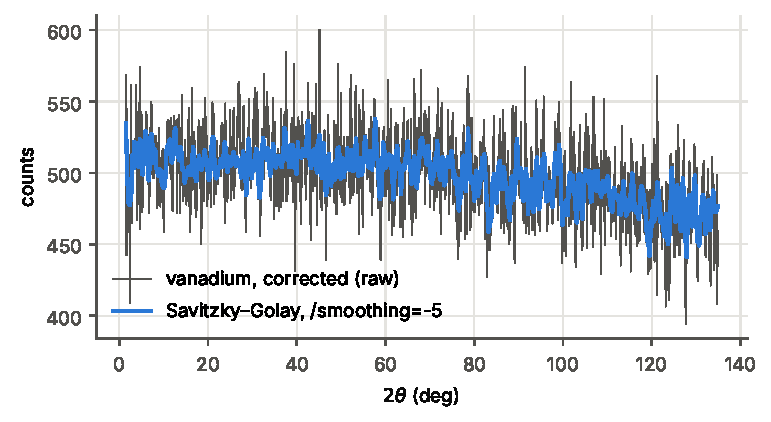
\includegraphics[width=0.85\linewidth]{figures/vanadium_smoothing.pdf}
  \caption{Vanadium after attenuation, multiple-scattering and Placzek
  corrections (grey) and after smoothing (blue). The V Bragg peaks are removed.}
  \label{fig:van}
\end{figure}

\section{Several detector groups}

\begin{com}
spectrum /to=8          ! blocks 1 to 8
\end{com}
or, for a selection,
\begin{com}
spectrum 1
spectrum 3
spectrum 5
\end{com}
The output file then contains one result block per spectrum, in the same order.

\section{Measurement in a furnace}

\begin{com}
furnace furnace.dat 1.0 1.04 /density=0.0722 /absorption=5.08 /scattering=4.95
vanadium vanadium.dat 0.3 /smoothing=-5 /furnace   ! vanadium measured in the furnace
background background.dat
\end{com}
The furnace factors $A_{h,\ldots}$ are now different from 1. Constraints
inherited from \cor: the beam must be narrower than the furnace inner diameter,
$R_3^2 - (w/2)^2 \geq R_2^2$, and $R_4^2-R_3^2 \leq R_1^2$.

\section{Calibration with the container}

If no \cmd{vanadium} command is given, the container is corrected for
attenuation, multiple scattering and Placzek, smoothed, and used instead. This
works when the container is made of a pure incoherent scatterer (vanadium):
\begin{com}
container can.dat 0.32 /type=v
! (no vanadium command)
\end{com}

\section{Flat-plate geometry}

\begin{com}
geometry plate 0                       ! plate normal along the beam
sample sample.dat 0.2 /density=0.0913  ! sample thickness 0.2 cm
container can.dat 0.3 /type=v          ! total thickness (walls + sample)
vanadium vanadium.dat 0.2 /smoothing=4 ! vanadium plate 0.2 cm
\end{com}
Multiple scattering is not corrected in plate geometry.

\section{Low-angle correction}

\begin{com}
low_angle 1.5 4 6 12 /vanadium /container
\end{com}
A line is fitted to vanadium + container between 6$^\circ$ and 12$^\circ$ and
the excess between 1.5$^\circ$ and 4$^\circ$ is subtracted. With
\cmd{cadmium}~\file{cd.dat} the cadmium data are used instead.

\section{Diagnostic output}

\begin{com}
write absorption calibration placzek
xout angle
title "Ni at 300 K"
\end{com}
The output file then contains the six attenuation factors, the corrected and
smoothed vanadium, and the Placzek correction, followed by the result as a
function of $2\theta$.

\section{Time-of-flight instrument}

\begin{com}
instrument sandals
xin wavelength                 ! the x column is wavelength (or tof, q)
range 0.3 2.7                  ! wavelength range kept (Angstrom)
beam 3 4
sample sam.dat 0.3 /density=0.05
component 1 si
container can.dat 0.32 /type=v
vanadium van.dat 0.3 /smoothing=1     ! cubic-spline smoothing
spectrum 1 40 10 1.0 /detector=h      ! block, 2theta, L1, L2, He detector
placzek series
output out.dat
execute /nolist
\end{com}
For TOF every correction is a function of wavelength; the attenuation factors are
computed at 21 wavelengths and fitted with a polynomial. The result is written in
increasing $Q$.

\section{Comparing with the original CORRECT}

\begin{com}
faithful on
@d4_example.com
\end{com}
reproduces the numbers of \cor\ 2.24. On the example the difference with the
default is a few tenths of a percent, mostly from the multiple scattering
(Chapter~\ref{chap:faithful}).

% =========================================================================
\chapter{Using pycorrect from Python}
\label{chap:python}
% =========================================================================

\section{The \code{Correct} object}

\begin{py}
from toscana.corrections.pycorrect import Correct

c = Correct(verbose=False, ask=False)   # no tables, no "Continue (Y/N)?"
c.run_file("d4_example.com")            # same as the command line
r = c.results[0]                        # results of the first spectrum
print(r["q"][:5], r["dcs"][:5])
\end{py}

Commands can also be given one by one with \code{c.command("...")}, and the
parameters can be changed directly in \code{c.st}, an object of class
\code{CorrectState} (Appendix~\ref{app:state}). For example, to study the effect
of the sample density:

\begin{py}
import numpy as np
from toscana.corrections.pycorrect import Correct

c = Correct(verbose=False, ask=False)
c.st.overwrite = True
for line in open("d4_example.com"):          # set-up without executing
    if not line.startswith(("execute", "output")):
        c.command(line)

for rho in (0.0913, 0.0900):
    c.st.sa_rho = rho
    c.command(f"output ni_rho{rho}.dat")
    c.command("execute /nolist")
    r = c.results[0]
    np.savetxt(f"ni_rho{rho}.txt", np.c_[r["q"], r["dcs"], r["err"]])
\end{py}

\section{Contents of the results}

\code{c.results} is a list with one dictionary per spectrum. All arrays are
NumPy arrays on the angle (two-axis) or wavelength (TOF) grid of the sample.

\begin{longtable}{@{}>{\raggedright\arraybackslash}p{5.2cm} >{\raggedright\arraybackslash}p{10.2cm}@{}}
\toprule
Key & Content \\
\midrule
\endhead
\code{block} & block number \\
\code{theta}, \code{q} & $2\theta$ (deg) and $Q$ (\AA$^{-1}$); TOF: \code{wav}, \code{q} \\
\code{dcs}, \code{err} & final $\dsig$ and its error (barn\,sr$^{-1}$\,atom$^{-1}$) \\
\code{assch}, \code{acsch}, \code{acch} & $A_{s,sch}$, $A_{c,sch}$, $A_{c,ch}$ of the sample set-up \\
\code{ahsch}, \code{ahch}, \code{ahh} & furnace factors $A_{h,sch}$, $A_{h,ch}$, $A_{h,h}$ \\
\code{avvch}, \code{acvch}, \code{acchv} & vanadium factors (and \code{ahvch}, \code{ahchv}, \code{ahhv}); TOF: \code{avvh} \\
\code{sample\_abs\_corrected} & $I_s$ after the Paalman \& Pings subtraction, before normalisation \\
\code{delta\_sa}, \code{delta\_va} & multiple-scattering ratio $\delta$ of sample and calibrant \\
\code{pc\_sa}, \code{pc\_va} & Placzek corrections of sample and calibrant \\
\code{calib\_raw}, \code{calib\_smooth} & corrected vanadium (or can) before and after smoothing \\
\bottomrule
\end{longtable}

\section{Calling the physics functions directly}

The two key functions can be used alone, without data files.

\subsection*{Attenuation factors}
\begin{py}
import math
from toscana.corrections.pycorrect import atcors

lam = 0.5
mu_s = 0.0913 * (18.5 + 4.49 * lam / 1.798)    # Ni, cm^-1
mu_c = 0.0722 * (4.95 + 5.08 * lam / 1.798)    # V
assch, acch, acsch, ahsch, ahch, ahh = atcors(
    math.radians(90.0),   # 2theta in radians
    0.30, 0.32,           # sample radius, can outer radius (cm)
    0.0, 0.0,             # furnace radii (r4 <= r3 -> no furnace)
    1.5,                  # beam width (cm)
    mu_s, mu_c, 0.0)      # total mu of sample, can, furnace
\end{py}
Without container give \code{r2 <= r1}; without furnace give \code{r4 <= r3}.
\code{plate(two\_theta\_rad, normal\_angle\_deg, t\_sample, t\_total, mu\_s, mu\_c)}
returns $(A_{s,sc}, A_{c,c}, A_{c,sc})$ for a slab.

\subsection*{Multiple scattering}
\begin{py}
from toscana.corrections.pycorrect import mscat
delta, delta2 = mscat(0.32, 5.0, mu_t, mu_scatt, return_details=True)
\end{py}
Arguments: radius, beam height, total and scattering linear coefficients.
\code{delta2} is the tabulated double/single ratio, \code{delta} the full
correction including $\mu_s/\mu_t$ and higher orders.

\subsection*{Tables for any geometry}
\file{examples/pp\_factors\_table.py}
prints all the factors every 5$^\circ$ (edit its \code{GEOMETRY} section):

\lstinputlisting[style=base,basicstyle=\ttfamily\scriptsize]{listings/pp_table_head.txt}

% =========================================================================
\chapter{Comparison with Monte Carlo simulations}
\label{chap:mc}
% =========================================================================

\pyc\ and a Monte Carlo trajectory code such as AMS address the same problem with
different approximations. A comparison is most informative quantity by quantity.

\section{Quantities to compare}

\begin{center}
\begin{tabularx}{\linewidth}{@{}lX@{}}
\toprule
\pyc & Monte Carlo equivalent \\
\midrule
$A_{s,sch}(2\theta)$ & singly scattered intensity from the sample into the detector at $2\theta$, with all bodies absorbing, divided by the same intensity with no attenuation \\
$A_{c,sch}$, $A_{c,ch}$ & the same for neutrons scattered once in the container, with and without the sample present \\
$A_{h,\ldots}$ & the same for the furnace \\
$\delta$ & (multiply scattered)/(singly scattered) intensity, averaged over angle \\
\code{sample\_abs\_corrected} & sample signal after the subtraction of container and furnace \\
\code{dcs} & final normalised cross-section \\
\bottomrule
\end{tabularx}
\end{center}

\section{Points to keep in mind}

\begin{itemize}
  \item \textbf{Same input.} Use the same $\mu_t(\lambda)$, $\mu_s$, radii, beam
        width and height in both codes. \pyc\ uses
        $\mu = n(\sigma_s + \sigma_a\lambda/1.798)$ with the values of
        \file{xsect.dat}.
  \item \textbf{2D geometry.} The Paalman \& Pings factors are computed in the
        horizontal plane for an infinitely tall cylinder; a simulation with a
        finite beam height and out-of-plane detectors can differ slightly.
  \item \textbf{Isotropic multiple scattering.} $\delta$ is a single number per
        sample (per wavelength in TOF), from a table computed for isotropic
        scattering; a simulation gives its angle dependence.
  \item \textbf{Narrow beam.} When the beam is narrower than the sample, the
        quadrature of \cor\ is accurate to about 0.4\%; the broad-beam case is
        accurate to better than 0.1\%.
  \item \textbf{Polynomial interpolation.} In a correction run the factors are a
        4th-degree polynomial through 10 angles; call \code{atcors} directly for
        the exact values.
  \item \textbf{faithful.} Compare with \code{faithful off}; use \code{on} only to
        understand differences with old \cor\ results.
\end{itemize}

% =========================================================================
\chapter{The \texttt{faithful} switch}
\label{chap:faithful}
% =========================================================================

During the translation several errors were found in \cor\ 2.24. By default
\pyc\ corrects them; \cmd{faithful on} reproduces them.

\begin{longtable}{@{}p{0.5cm} >{\raggedright\arraybackslash}p{3.2cm} >{\raggedright\arraybackslash}p{5.4cm} >{\raggedright\arraybackslash}p{5.4cm}@{}}
\toprule
\# & Where & \cor\ 2.24 (\code{faithful on}) & Default (\code{faithful off}) \\
\midrule
\endhead
1 & multiple scattering & no interpolation in $R/H$ (grid value below is used) & bilinear interpolation in $(\mu R, R/H)$ \\
2 & can as calibrant & $\sigma_s$ and $\sigma_a$ passed where $\mu_t$ and $\mu_s$ are expected & correct arguments \\
3 & low-angle correction & only the slope divided by $n_{\text{fit}}$; background error taken from the furnace & whole fit divided; background errors \\
4 & vanadium in furnace/can & error coefficients not squared & squared \\
5 & polynomial smoothing & error bars used as weights & weights $1/e^2$ \\
6 & Savitzky--Golay & Bragg peaks at the detector edges not skipped & skipped \\
7 & fullness & error not propagated & propagated \\
8 & \cmd{placzek diatomic} & $\omega$ read from the wrong parameter (always 0) & second parameter \\
9 & TOF wavelength cut & errors replaced by counts, $x$ not shifted & errors kept, $x$ shifted \\
10 & TOF vanadium in furnace & furnace error subtracted in quadrature & added \\
11 & flat plate (\code{PLATE}) & reflection: $A_{c,sc}$ of the back window without the sample on the way out; $2\theta=0$ at normal incidence: $A_{c,c}$ is the sum of the two windows ($\times 2$) & sample and front window in and out, $e^{(\mu_c d+\mu_s t)(b-a)}$; mean of the two windows \\
\bottomrule
\end{longtable}

\begin{warn}[Always corrected]
A few faults cannot be reproduced because they depended on uninitialised memory:
the undefined array written by \cmd{write absorption}, a furnace factor used
before being computed (TOF), and $0/0$ in the diatomic Placzek correction when
$\omega=0$. The time-of-flight chain of the PC version of \cor\ could not run at
all (it requested the VAX binary format); in \pyc\ it works with TEXT files.
\end{warn}

% =========================================================================
\chapter{Troubleshooting}
% =========================================================================

\begin{description}[style=nextline,leftmargin=0.5cm]
\item[\code{FileExistsError: An output file already exists}]
  Delete the output file, choose another name, or set
  \code{c.st.overwrite = True} in Python.
\item[Nothing is computed after \cmd{execute}]
  No \cmd{spectrum} command was given.
\item[\code{ZeroDivisionError} or infinite values]
  The sample density is missing (\code{/density}), or a radius is zero.
\item[\code{ValueError: ATCORS: the beam is wider than the furnace i.d.}]
  Reduce the beam width or check the furnace radii (they are inner and outer radii, not diameters).
\item[\code{Symbol "xx" not found}]
  Check the symbol in \file{xsect.dat} (lower case, e.g.\ \code{d} for deuterium),
  or give weight and cross-sections explicitly.
\item[\code{COMMENT - outside range tabulated}]
  $\mu R > 9.5$ or $R/H$ outside 0.05--1: $\delta_2$ is computed by direct
  integration (slower, but correct).
\item[Wrong file read]
  File names are relative to the current folder, not to the \file{.com} file.
\end{description}

% =========================================================================
\appendix
\chapter{Correspondence with the Fortran sources}
\label{app:corr}
% =========================================================================

\begin{longtable}{@{}>{\raggedright\arraybackslash}p{3.5cm} >{\raggedright\arraybackslash}p{5.5cm} >{\raggedright\arraybackslash}p{6.0cm}@{}}
\toprule
Fortran file & Routine & Python \\
\midrule
\endhead
\file{correct\_224.f} & \code{PROGRAM CORRECT} & \code{correct.main}, \code{Correct.run\_file}, \code{.interactive} \\
 & \code{BLOCK DATA} & defaults of \code{state.CorrectState} \\
 & \code{OBEY\_LINE}, \code{CORRECT\_LIST} & \code{Correct.obey\_line}, \code{Correct.correct\_list} \\
 & \code{READ\_ATOM\_DATA} & \code{correct.read\_atom\_data} \\
\file{correct\_224.inc} & COMMON blocks & \code{CorrectState}, \code{Species}, \code{Spectrum}, \code{Collimator} \\
\file{parse\_line.f} & \code{PARSE\_LINE} & \code{parse\_line.parse\_line} \\
\file{correct\_2axis\_\allowbreak 224.f} & \code{CORRECT\_2AXIS}, \code{ABSOR} & \code{correct\_2axis.\allowbreak correct\_2axis}, \code{absor} \\
 & \code{SMOOTH\_VANADIUM}, \code{SMOOTH\_VANADIUM\_SG}, \code{SMOOTH}, \code{QUADFIT2} & \code{smooth\_vanadium}, \code{smooth\_vanadium\_sg}, \code{\_sg\_smooth}, \code{\_quadfit2} \\
 & \code{PLACZEK} & \code{correct\_2axis.placzek} \\
\file{correct\_tofdif\_\allowbreak 224.f} & \code{CORRECT\_TOF}, \code{NORM}, \code{ABSORB}, \code{MULSCAT} & \code{correct\_tof}, \code{norm\_to\_monitor}, \code{absorb}, \code{mulscat} \\
 & \code{SPLINE\_SMOOTH}, \code{PLAMOL}, \code{PLAATOM}, \code{LITLF}, \code{BIGF} & same names \\
\file{ndplib.f} & \code{ATCORS}, \code{ATCOR\$GXY3}, \code{GXY3x}, \code{GXY3z}, \code{ATCOR\$F1}--\code{F17}, \code{G1}--\code{G19} & \code{atcors}, \code{\_AtcorsIntegrator} (methods \code{gxy3}, \code{gxy3\_beam}, \code{F1}--\code{F17}, \code{G1}--\code{G19}) \\
 & \code{VIS}, \code{TRANS}, \code{AREA}, \code{BEAMWX/Z} & \code{\_vis}, \code{\_trans}, \code{area}, \code{\_beamw} \\
 & \code{MSCAT}, \code{MULSCS}, \code{H2EL} & \code{mscat}, \code{mulscs}, \code{h2el} \\
\file{routines.f} & \code{PLATE}, \code{POLYFIT} & \code{routines.plate}, \code{routines.polyfit} \\
\file{fileio.f} & \code{READ\_FILE}, \code{OPEN/APPEND/CLOSE\_FILE} & \code{fileio.read\_file}, \code{DataWriter} \\
\file{harwell.f} & \code{VB01S} (+ helpers) & \code{numpy.linalg.lstsq} \\
 & \code{VB06A}, \code{TG01B} & \code{harwell.lsq\_cubic\_spline} (SciPy) \\
\bottomrule
\end{longtable}

\chapter{Parameters of \texttt{CorrectState}}
\label{app:state}

\begin{longtable}{@{}>{\raggedright\arraybackslash}p{5.2cm} >{\raggedright\arraybackslash}p{3.0cm} >{\raggedright\arraybackslash}p{6.8cm}@{}}
\toprule
Attribute & Default & Meaning (set by command) \\
\midrule
\endhead
\code{files} & empty & dict: \code{sample}, \code{container}, \code{furnace}, \code{vanadium}, \code{bkg\_*}, \code{cadmium}, \code{output}, \code{cs\_file} \\
\code{instrument}, \code{inst\_type} & D4, 2-AXIS & \cmd{instrument} \\
\code{wavelength} & 0.7 & \cmd{wavelength} \\
\code{beam\_height}, \code{beam\_width} & 3.0, 1.5 & \cmd{beam} \\
\code{geometry} & CYLINDRICAL & \cmd{geometry} \\
\code{ca\_r1}, \code{ca\_r2} & 0, 0 & sample radius, can outer radius \\
\code{fu\_r1}, \code{fu\_r2}, \code{va\_r} & 0 & furnace radii, vanadium radius \\
\code{sa\_rho}, \code{sa\_temp}, \code{sa\_fullness} & 0, 300, 1 & \cmd{sample} qualifiers \\
\code{ca\_rho}, \code{ca\_abs\_cs}, \code{ca\_scat\_cs} & 0.0722, 5.08, 4.95 & container (V) \\
\code{fu\_*}, \code{va\_*} & V values & furnace, vanadium \\
\code{species} & [] & list of \code{Species} (\cmd{component}) \\
\code{spectra} & [] & list of \code{Spectrum} (\cmd{spectrum}) \\
\code{vanadium\_smoothing} & 0 & \code{/smoothing} \\
\code{placzek\_correction}, \code{omegav} & NONE, 0 & \cmd{placzek} \\
\code{lowang}, \code{low\_*} & 0, False & \cmd{low\_angle} \\
\code{calib\_ur/vr/wr} & 2.595, $-$2.207, 0.709 & \cmd{calibration} \\
\code{xouttype}, \code{xtype} & Q, WAVELENGTH & \cmd{xout}, \cmd{xin} \\
\code{wav\_min}, \code{wav\_max}, \code{monitor\_spectrum} & 0.1, 3.0, 0 & TOF \\
\code{collimator} & disabled & \cmd{collimator} \\
\code{faithful} & False & \cmd{faithful} \\
\code{overwrite} & False & allow overwriting the output file \\
\code{data\_format} & TEXT & input format (TEXT or DATA) \\
\bottomrule
\end{longtable}

% =========================================================================
\begin{thebibliography}{9}
\bibitem{pp} H.~H.~Paalman and C.~J.~Pings, \emph{J. Appl. Phys.} \textbf{33}, 2635 (1962).
\bibitem{ba} I.~A.~Blech and B.~L.~Averbach, \emph{Phys. Rev.} \textbf{137}, A1113 (1965).
\bibitem{yarnell} J.~L.~Yarnell, M.~J.~Katz, R.~G.~Wenzel and S.~H.~Koenig, \emph{Phys. Rev. A} \textbf{7}, 2130 (1973).
\bibitem{sg} A.~Savitzky and M.~J.~E.~Golay, \emph{Anal. Chem.} \textbf{36}, 1627 (1964).
\end{thebibliography}

\end{document}
